
\chapter{Теорема Гливенко-Кантелли. Метод подстановки} % (fold)

\section{Теорема Гливенко-Кантелли}\label{lec:3/sec:1}

Пусть  $X=(X_1, \dots, X_n)$ - случайный вектор наблюдений. Дальше $n$ будет расти. Поэтому предполагается, что на некотором вероятностном пространстве $(\Omega, \mathcal{F}, P)$ определена бесконечная последовательность н.о.р. случайных величин $X_1, X_2, \dots$ с неизвестной функцией распределения $F(x)$. Наблюдение $X$ содержит первые $n$ компонент этой последовательности.

Наша цель - оценить $F(x) = P(X_1 \leq x), x \in \mathbb{R}$. Зафиксируем $\omega \in \Omega$ и рассмотрим реализации $\displaystyle x_k = X_k(\omega), \;k=1,\dots, n$.
Пусть $\displaystyle x_{(1)}\leq x_{(2)} \leq \dots\leq x_{(n)}$.
\begin{definition}
	Случайная величина $X_{(k)}$, равная на упомянутом $\omega$
	$\displaystyle X_{(k)}(\omega)= x_{(k)}, \;k = 1, 2, \dots, n$
	называется \red{к-ой порядковой статистикой}.
	Совокупность $\displaystyle X_{(1)}\leq X_{(2)} \leq...\leq X_{(n)}$
	называется \red{вариационным рядом}.
\end{definition}

\begin{definition}
	Оценкой $F(x)$ в точке $x$ возьмем $\hat{F}_n(x) = \frac{1}{n}\sum\limits_{i=0}^{n}I(X_i \leq x)$, где $I$ - индикатор.
	$\hat{F}_n(x)$ называется \red{эмпирической функцией распределения}.
\end{definition}

Если $x_{(1)}\leq x_{(2)} \leq \dots \leq x_{(n)}$ - реализация вариационного ряда, то график реализации $\hat{F}_n(x)$ такой:
\begin{multicols}{2}

	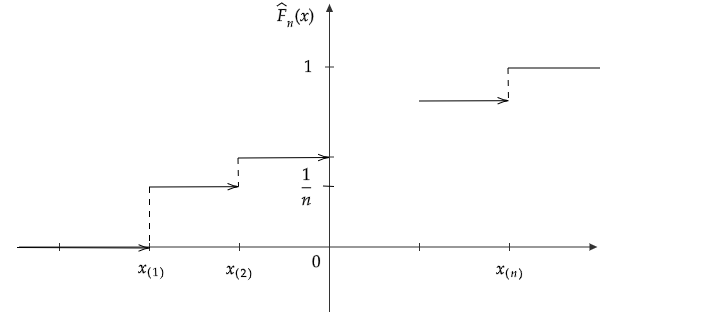
\includegraphics[height=5cm,width=10cm]{lec3im1}

	\columnbreak
	\hfill \break

	При каждом $\omega$ $\hat{F}_n(x) =\hat{F}_n(x, \omega)$ - дискретная ф.р. 

	При фиксированном $ x \;\; \hat{F}_n(x)$ - случайная величина.
\end{multicols}

В силу УЗБЧ: $\displaystyle \frac{1}{n}\sum\limits_{i=0}^{n}I(X_i \leq x) \xrightarrow[n \to \infty]{\text{п.н.}} EI(X_1 \leq x) = F(x)$.

В силу ЦПТ: $\displaystyle \frac{1}{n}(\hat{F}_n(x)- F(x))=\frac{1}{\sqrt{n}}\sum\limits_{i=0}^{n}(I(X_i \leq x)- F(x)) \;\xrightarrow[n \to\infty]{d}  N(0, \hat{F}_n(x)- F^2(x))$, т.к. $ DI(X_1 \leq x) = EI^2(X_1 \leq x) -(EI(X_1 \leq x))^2 = F(x) - F^2(x)$.
\vspace{1cm}

Докажем следующую важнейшую теорему:

\begin{theorem}[\red{Гливенко-Кантелли}]
	Пусть $X_1, \dots, X_n$ - н.о.р.с.в., $X_1 \sim F(x)$. Тогда 
	$$ \sup\limits_x|\hat{F}_n(x)-F(x)| \xrightarrow[n\to\infty]{\text{п.н.}}
	0$$
\end{theorem}
\begin{Proof}
	Пусть $F(x)$ непрерывна. Пусть $\varepsilon > 0$ - любое малое число, такое что $N = \frac{1}{\varepsilon}$ - целое. Выберем точки $\displaystyle -\infty= z_0<z_1< \dots < z_{N-1}<z_N=\infty$
	так что $\displaystyle F(z_k) = \frac{k}{N}, k = 0,1, \dots,N$. 
	Для $x \in [z_k, z_{k+1})$ в силу монотонности $\hat{F}_n(x)$ имеем:
	$$\hat{F}_n(x) - F(x)\leq \hat{F}_n(z_{k+1})-F(z_k) = \hat{F}_n(z_{k+1})- F(z_{k+1}) + \varepsilon \leq \max\limits_k|\hat{F}_n(z_{k}) - F(z_k)| + \varepsilon$$
	$$\hat{F}_n(x) - F(x) \geq  \hat{F}_n(z_{k})-F(z_{k+1}) = \hat{F}_n(z_{k}) - F(z_k) - \varepsilon \geq -\max\limits_k|\hat{F}_n(z_{k}) - F(z_k)| + \varepsilon$$
	Из двух последних неравенств получаем:
	$$\sup\limits_x|\hat{F}_n(x) - F(x)| \leq \max\limits_k|\hat{F}_n(z_{k}) - F(z_k)| + \varepsilon \eqno(1)$$
	Пусть $\displaystyle A_k = \{ \omega : \hat{F}_n(z_{k}) \rightarrow F(z_k) \}$. Тогда $\displaystyle P(A_k) = 1$. Пусть $\displaystyle A = \bigcap\limits_kA_k$. Тогда $\displaystyle \forall \omega \in A \; \max\limits_k|\hat{F}_n(z_{k}) - F(z_k)|\to 0$. Значит: 
	$$\forall \omega \in A \; \exists n_0=n_0(\omega): \; n > n_0 \;\; \max\limits_k|\hat{F}_n(z_{k}) - F(z_k)|<\varepsilon\eqno(2)$$
	В силу (1) и (2) для этого $\omega$ при $n>n_0$ получаем, что:
	$$\sup\limits_x|\hat{F}_n(x) - F(x)| < 2\varepsilon\eqno(3)$$
	Так как $P(A)=1$ и $\varepsilon$ произвольно, то (3) означает $\displaystyle \sup\limits_x|\hat{F}_n(x) - F(x)| \xrightarrow[n\to\infty]{\text{п.н.}}0$.
\end{Proof}

\begin{problem}
	Доказать теорему Гливенко-Кантелли для разрывной $F(x)$.
\end{problem}
$($см. [А.А.Боровков. Математическая статистика. Оценка параметров и проверка гипотез. М., Наука, 1984 г.]$)$

\section{Метод подстановки}\label{lec:3/sec:2}
Пусть надо оценить параметр $\theta = G(F)$, $G(\cdot)$ - функционал на множестве функций распределения. Естественная оценка подставновки $\displaystyle \hat{\theta}_n = G(\hat{F}_n)$.

\begin{example}
	Пусть $\displaystyle E|X_1|^k<\infty,\;\; \nu_k=EX_1^k,\; k\in \mathbb{N}$. $\nu_k$ называют \red{к-ым начальным моментом}. Тогда $\displaystyle \nu_k = G(F) = \int\limits^{\infty}_{-\infty}x^kdF(x)$.
	Оценка подстановки для $\theta = \nu_k$: $\displaystyle \;\;\;\;\; \hat{\theta}_n = \hat{\nu}_k = \int\limits^{\infty}_{-\infty}x^kd\hat{F}_n(x) = \frac{1}{n}\sum\limits_{i=1}^{n}X_{(i)}^k = \frac{1}{n}\sum\limits_{i=0}^{n}X_i^k$.\\
	В силу УЗБЧ: $\displaystyle \;\;\;\;\; \hat{\nu}_k = \frac{1}{n}\sum\limits_{i=0}^{n}X_i^k \xrightarrow[n\to\infty]{\text{п.н.}} EX_1^k=\nu_k$.\\
	Кроме того, при $EX_1^{2k} < \infty$ имеем в силу ЦПТ:
	$$\sqrt{n}(\hat{\nu}_k - \nu_k) =\frac{1}{\sqrt{n}}\sum\limits_{i=1}^{n}(X_i^k-\nu_k) \xrightarrow{d}\; N(0, \nu_{2k} - \nu_k^2),\;n\rightarrow\infty$$  
	Значит $\displaystyle (\nu_{2k} - \nu_k^2)^{-\frac{1}{2}}\sqrt{n}(\hat{\nu}_k - \nu_k) \rightarrow N(0,1)$. Отсюда:
	$$\forall \varepsilon >0 \; P\left((\nu_{2k} - \nu_k^2)^{-\frac{1}{2}}|\sqrt{n}(\hat{\nu}_k - \nu_k)| \leq \varepsilon\right)\rightarrow\Phi(\varepsilon)-\Phi(-\varepsilon) =2\Phi(\varepsilon)-1 \eqno(4)$$
	где $ \Phi(x)=\frac{1}{\sqrt{2\pi}}\int\limits^{\infty}_{-\infty}e^{-\frac{t^2}{2}}dt$ - функция Лапласа.
	Асимптотическая нормальность позволила оценить в $(4)$ точность оценки $\hat{\nu}_k$.
\end{example}

\begin{example}[\blue{Выборочные квантили}]
	Для $0<p<1$ и любой (не обязательно непрерывной) функции распредления $F(x)$ полагают $\displaystyle F^{-1}(p) \equiv \sup{x: F(x) \leq p}$.
	Величина $F^{-1}(p)$ называется \red{квантилью} функции распределения $F(x)$ и обозначается далее $\xi_p$.

	Если $F(x)$ непрерывна и строго возрастает, то $F(\xi_p) = p$.
\end{example}

Пусть $\displaystyle X_{(1)}\leq X_{(2)} \leq \dots \leq X_{(n)}$
- вариационный ряд выборки $X_1, \dots, X_n$. Оценка $\xi_p$ по методу подстановки:
$$\hat{\xi}_p = \hat{F}_n^{-1}(p) = sup\{x: \hat{F}_n{x} \leq p \} = X_{([np]+1)}$$

\begin{lemma}
	Пусть функция распределения $F(x)$ непрерывна и строго возрастает. Тогда функционал $G(F) = \xi_p, \; 0<p<1$ непрерывен в равномерной метрике. Т.е., если последовательность ф.р. ${F_n(x)}$ такова, что $\displaystyle \sup\limits_x|F_n(x) - F(x)|\rightarrow0$, то $\displaystyle G(F_n)\rightarrow G(F)$.
\end{lemma}
\begin{Proof}
	$\forall\;\varepsilon>0$ при $n>n_0(\varepsilon)$ имеем:
	$$\begin{gathered}
		G(F_n) \equiv \xi_p^n = \sup{x: F_n(x) \leq p} = \sup{x: F(x) \leq F(x) - F_n(x)+p}\leq \\ 
		\le \sup{x: F(x) \leq \sup\limits_y|F_n(y)-F(y)|+p} \leq \sup{x: F(x)\leq p+\varepsilon} = F^{-1}(p+\varepsilon) 
	\end{gathered}$$
	Аналогично: $\displaystyle \xi_p^n \geq F^{-1}(p-\varepsilon),\;n>n_0$. Значит $\displaystyle F^{-1}(p-\varepsilon)\leq\xi_p^n\leq F^{-1}(p+\varepsilon),\;n>n_0$. Тогда $\displaystyle F^{-1}(p-\varepsilon)\leq \underset{n\to\infty}{\underline{\lim}}\xi_p^n\leq \underset{n\to\infty}{\overline{\lim}}\xi_p^n \leq F^{-1}(p+\varepsilon)$.
	Функция $F^{-1}(t),\;0<t<1$ непрерывна. Устремляя $\varepsilon$ к нулю получим:
	$$\xi_p=\underline{\lim}_{n\rightarrow\infty}\xi_p^n\leq\overline{\lim}_{n\rightarrow\infty}\xi_p^n=\xi_p, \text{ т.е. } \lim\limits_{n\rightarrow\infty}\xi_n^p=\xi_p$$
\end{Proof}

\begin{conseq}
	Если $F(x)$ непрерывна и строго возрастает, то $\displaystyle \hat{\xi}_p \xrightarrow[n\rightarrow\infty]{\text{п.н.}} \xi_p$. Это прямо следует из \blue{теоремы Гливенко-Кантелли}.
\end{conseq}
\begin{definition}
	Величина $\xi_{\frac{1}{2}}$ называется \red{медианой}, а $\hat{\xi}_{\frac{1}{2}}$- \red{ выборочной медианой}.
\end{definition}

\begin{theorem}
	Пусть $F(x)$ дифференциируема в точке $\xi_{\frac{1}{2}}$, и $g(\xi_{\frac{1}{2}})\equiv F'(\xi_{\frac{1}{2}})>0$. Тогда:
	\[\sqrt{n}(\hat{\xi}_{\frac{1}{2}}-\xi_{\frac{1}{2}})\xrightarrow{d}N(0,\frac{1}{4g^2(\xi_{\frac{1}{2}})}),\;\;n\rightarrow\infty. \]
\end{theorem}

\section{Асимптотическая относительная эффективность оценок (АОЭ)}\label{lec:3/sec:3}

Асимптотически нормальные оценки можно сравнивать между собой.

Пусть по вектору наблюдений $X = (X_1, \dots, X_n)$ оценивается параметр $\theta$, и $\hat{\theta}_{1n}$ - его оценка. Пусть
$$\sqrt{n}(\hat{\theta}_{1n} - \theta) \xrightarrow[n\to\infty]{d} N(0, \sigma^2(\theta))\eqno(5)$$
Пусть есть другая оценка $\hat{\theta}_{2n}$, такая что:
$$\sqrt{n}(\hat{\theta}_{1n'} - \theta) \xrightarrow[n\to\infty]{d} N(0, \sigma^2(\theta))\eqno(6)$$
где $n'=n'(n) \xrightarrow[n\to\infty]{} \infty$.

\begin{definition}
	\red{Асимптотической относительной эффективностью} (АОЭ) оценки $\hat{\theta}_{1n}$ относительно оценки $\hat{\theta}_{2n}$ называется величина
	\[l_{1,2} \equiv \lim\limits_{n\rightarrow\infty}\frac{n'(n)}{n}.\]
\end{definition}

Пусть, например, $l_{1,2}=3$ . Тогда при больших $n$ $n'\approx3n$. Значит, для $\hat{\theta}_{2n}$ нужно в три раза больше наблюдений, чем для $\hat{\theta}_{1n}$, чтобы достичь одинаковой точности $\sigma^2(\theta)/n$. Оценка $\hat{\theta}_{1n}$ в три раза лучше оценки $\hat{\theta}_{2n}$.

\begin{lemma}
	Пусть $\displaystyle \sqrt{n}(\hat{\theta}_{in} - \theta)\xrightarrow[n\to\infty]{d}N(0,\sigma^2_i(\theta)),\; \sigma^2_i(\theta)>0, \; i = 1,2$.
	Тогда АОЭ существует и равна
	\[l_{1,2} = \frac{\sigma^2_2(\theta)}{\sigma^2_1(\theta)}.\]
\end{lemma}

\begin{proof}
	Пусть $n'\sim \frac{\sigma^2_2(\theta)}{\sigma^2_1(\theta)}n,\;\;n\rightarrow\infty$. Тогда
	$$\begin{gathered}
		\sqrt{n}(\hat{\theta}_{2n'}-\theta) = \sqrt{\frac{n}{n'}}\sqrt{n'}(\hat{\theta}_{2n'}-\theta) \xrightarrow{d} \frac{\sigma_2(\theta)}{\sigma_1(\theta)}\xi, \;\;\xi\sim N(0,\sigma^2_2(\theta)) \\
		(\text{использовали \blue{лемму Слуцкого}: если } \xi_n \xrightarrow{d}\xi,\; \eta_n \xrightarrow{d} c, \text{ то }\xi_n\eta_n \xrightarrow{d} c\xi)
	\end{gathered}$$
	Значит: $\displaystyle \sqrt{n}(\hat{\theta}_{2n'}-\theta) \xrightarrow{d} N(0,\sigma^2_1(\theta))$. Получаем: $\displaystyle \lim\limits_{n\rightarrow\infty} \frac{n'(n)}{n}=\frac{\sigma^2_2(\theta)}{\sigma^2_1(\theta)}$.
\end{proof}

\begin{example}[Важный]
	Пусть $\displaystyle X_i = \theta + \varepsilon_i, \;\; i=1,..,n,\;\; {\varepsilon_i}-\text{ н.о.р.}$. Пусть $\displaystyle E\varepsilon_1 = 0, \;\; D\varepsilon_1 = \sigma^2 < \infty$. Тогда $EX_1 = \theta$, и оценкой $\theta$ можно взять $\overline{X}= \frac{1}{n}\sum\limits_{i=1}^{n}X_i$. Знаем, что $\displaystyle \sqrt{n}(\overline{X}- \theta) \xrightarrow[n\to\infty]{d} N(0, \sigma^2)$, т.к. $\nu_2- \nu_1^2 = \sigma^2$.
\end{example}

Пусть теперь $\varepsilon_1$ имеют ф.р. $G(x)$ и существует плотность вероятности $g(x) = G'(x)$. Пусть $g(x) = g(-x)$ и $g(0)>0$. Тогда $G(0)=\frac{1}{2}$. Значит ф.р. $X_1$ имеет вид: $\displaystyle \;\;\; P(X_1 \leq \theta) = P(\theta+\varepsilon_1 \leq \theta) = P(\varepsilon_1 \leq 0) = \frac{1}{2}$, т.е. $\theta$-медиана $X_1$.

Возьмем оценкой выборочную медиану $\hat{\xi}_{\frac{1}{2}}$. Тогда 
$\displaystyle \sqrt{n}(\hat{\xi}_{\frac{1}{2}}-\theta)\xrightarrow[n\to\infty]{d}N\left(0,\frac{1}{4g^2(0)}\right)$, т.к. плотность вероятности $X_1$ есть $g(x-\theta)$, и $\displaystyle g(x-\theta)|_{x=\xi_{\frac{1}{2}}=\theta} = g(0)$.

Значит, АОЭ выборочной медианы относительно выборочного среднего равна 
\[l_{\hat{\xi}_{\frac{1}{2}}, \overline{X}}= \dfrac{\sigma^2}{\frac{1}{4g^2(0)}} = 4g^2(0)\sigma^2.\]
\begin{itemize}
	\item[$1)$] 
		Если $\varepsilon_1 \sim N(0, \sigma^2)$ , то
		$\displaystyle l_{\hat{\xi}_{\frac{1}{2}}, \overline{X}} = 4\left(\frac{1}{\sqrt{2\pi}\sigma}\right)^2\sigma^2= \frac{2}{\pi}\approx0.637<1$. Т.е. если выборочную медиану построить по $n$ наблюдениям, то ту же точность получим для $\overline{X}$ по $0.637n$ наблюдениям! $\; \overline{X}$ - лучше выборочной медианы в $\frac{\pi}{2}$ раз.
	\item[$2)$] 
		Пусть $\varepsilon_1 \sim Lap(\lambda), \;\; \lambda>0$. Тогда 
		$\displaystyle g(x) = \frac{\lambda}{2}e^{-\lambda|x|}$. $\displaystyle E\varepsilon_1 = 0, E\varepsilon_1^2 = \frac{2}{\lambda^2}$. $\displaystyle l_{\hat{\xi}_{\frac{1}{2}}, \overline{X}} = 4\left(\frac{\lambda}{2}\right)^2 \frac{2}{\lambda^2} = 2 > 1$.
		Отсюда, медиана в 2 раза лучше выборочного среднего.
\end{itemize}

% subsection асимптотическая_относительная_эффективность_оценок_ (end)

% subsubsection subsubsection_name (end)
% chapter теорема_глиненко_кантелли_метод_подстановки (end)